\chapter*{Introducción}
\addcontentsline{toc}{chapter}{Introducción}

% =====================Estilo de página================================
\pagestyle{fancy}
\fancyhf{} % clear all header fields
\fancyhead[LE]{\nouppercase{\textbf{Introducción} \hfill}}
\fancyhead[RO]{\nouppercase{\hfill \textbf{Introducción}}}
\fancyfoot[LE]{\nouppercase{\thepage \hfill \emph{Pressure Distribution Inside Nucleons in a
Tsallis-MIT Bag Model}}}
\fancyfoot[RO]{\nouppercase{\emph{Pressure Distribution Inside Nucleons in a
Tsallis-MIT Bag Model} \hfill \thepage}}
% =====================================================================

% 12 345.678 90                     \num{12345,67890} \\
% 0.3 ×1045                         \num{.3e45} \\
% 1 ±2i                             \complexnum{1+-2i}
% 1.654 ×2.34 ×3.430                \numproduct{1.654 x 2.34 x 3.430}
% kg m s−1                          \unit{kg.m.s^{-1}}
% kg m s−1                          \unit{\kilogram\metre\per\second} 
% kg m/s                            \unit[per-mode = symbol]{\kilogram\metre\per\second}
% kg m/(A s)                        \unit[per-mode = symbol]{\kilogram\metre\per\ampere\per\second}
% 
% \Gls{maths}

Según el modelo de \acrfull{qcd} las partículas hadrónicas están compuestas por quarks, los cuales permanecen confinados dentro de los hadrones. Este confinamiento es una de las características fundamenales de la \acrshort{qcd} y es una de las razones por las cuales no se han observado quarks libres en la naturaleza.

% Renombrando las figuras
\renewcommand{\figurename}{Fig.}

\begin{wrapfigure}{r}{0.45\textwidth}
\centering
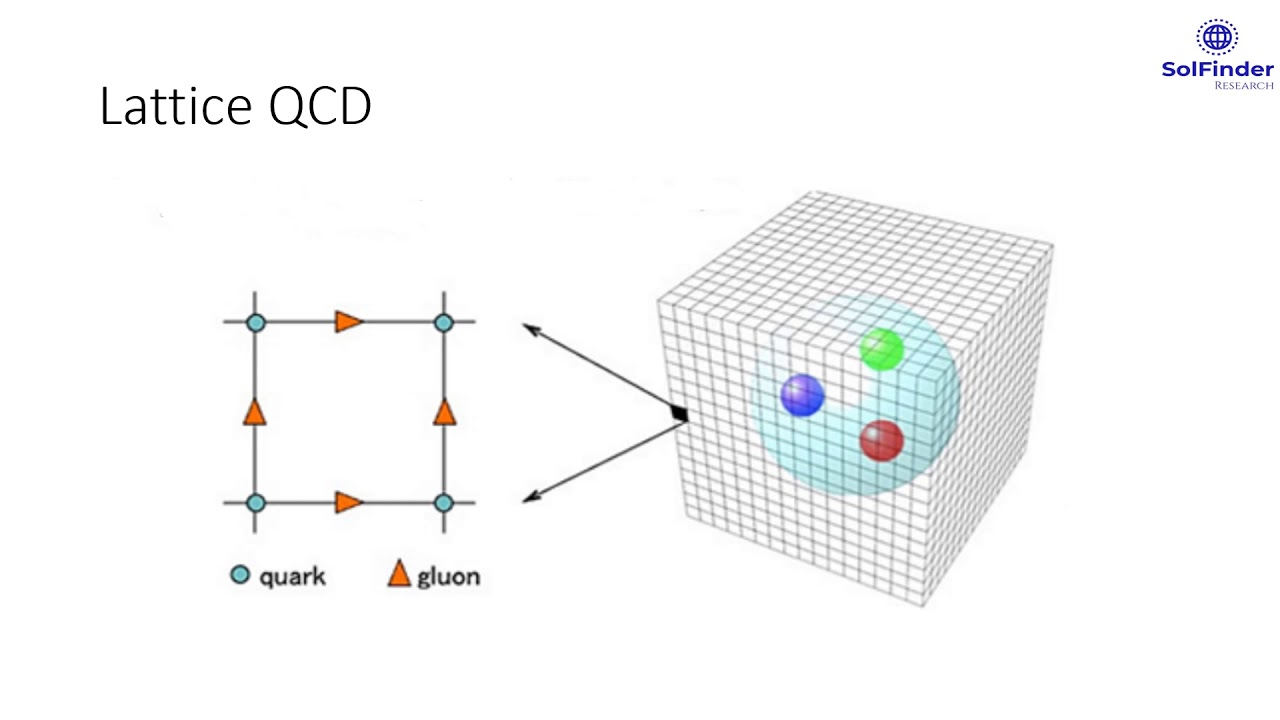
\includegraphics[width=0.4\textwidth]{./Images/LQCD.jpg}
\caption[Red LQCD]{\emph{Diagrama de red tipo LQCD en donde los nodos se encuentran donde los quarks y las aristas representan campos gluónicos}}
\label{fig: LQCD}
\end{wrapfigure}

%Over the years, various phenomenological descriptions of proton structures have been proposed, such as string models [1,2], which depict hadrons as oscillating strings; bag models, which consider quarks confined within a cavity; and valon models
A través de los años hemos desarrollado miles de modelos para describir la estructura del protón, por ejemplo en \cite{Artru1974, Andersson_1983} se describe hadrones como cuerdas oscilantes, modelos de bolsa como en \cite{AIHPA_1968__8_2_163_0,DeTar_1983}, que considera quarks confinados en una cavidad, y modelos de valones \cite{Hwa_1981}.

Con el fin de explorar la física de materia quark, se han desarrollado varias técnicas que permiten vislumbrar los efectos de ese tipo de interacciones como por ejemplo \acrfull{lqcd}; y por otro lado, se han desarrollado modelos que pueden bosquejar este tipo de interacciones a partir de simplificaciones como sucede en el modelo de bolsa (\acrfull{bm}), el modelo de cuerdas, el modelo de partones y un largo etcétera\cite{DeTar_1983}, puesto que ocurren interacciones no lineales dentro de los hadrones. 

%Lattice QCD computations provide reliable results of hadron structures that con- tain heavy quarks and have recently been used as state-of-the-art calculations by the HAL-QCD collaboration[6,7]. The description obtained by HAL QCD of the final state strong interactions between proton–neutron and proton–hyperons systems was compared to the experimental results published by the ALICE Collaboration 

Cálculos de \acrshort{lqcd} proporcionan resultados confiables de estructuras hadrónicas que contienen quarks pesados y ha sido recientemente usadas como cálculos de estado de arte por la colaboración HAL-QCD \cite{Iritani_2019,Hatsuda_2017}. La descripción obtenida por HAL QCD de los estados finales de interacciones fuertes entre sistemas protón-neutrón y protón hiperones fue comparado a los resultados experimentales publicados por la colaboración ALICE \cite{Collaboration2020, Collaboration2021}

\qty{10}{cm}

\num{1.2304} \unit{\candela}

\acrshort{lqcd} consiste en una técnica numérica que lleva a cabo gran cantidad de cálculos en una red espacio - temporal Euclídea muy grande (los parámetros de red $a$ son del orden de $\mathit{\unit{\femto\meter}}$ o como se menciona en [INTRO A LQCD], en un rango de $2 \, \unit{GeV} \leq {a}^{-1} \leq 5 \, \unit{GeV}$), Fig.~\ref{fig: LQCD}. Debido a que ocupa redes con millones de nodos, la dificultad de este tipo de modelos recae en la cantidad de cálculos necesarios para resolver dichos modelos. 
Partiendo de esto, se tiene un nuevo problema: \emph{el problema del signo} [más referencias], el cual surge en simulaciones Monte Carlo como las que se ocupan para resolver \acrshort{lqcd}, esto consiste en que el peso de las configuraciones de simulaciones cuánticas Monte Carlo se vuelven negativas o incluso complejas, y por lo tanto, no pueden ser interpretadas como proabilidades clásicas[Sign problem in QMC simulation]. 

NOTA: Hablar acerca del operador de Dirac no hermitiano

Los cálculos de \acrshort{lqcd} 

han conseguido resultados fiables acerca de las estructuras de hadrones que contienen quarks pesados


NOTA: Hablar acerca de resultados obtenidos con LQCD

Hemos propuesto un modelo que se basa en el modelo de bolsa (\acrshort{bm}) del \acrfull{mit} [add ref] y estadística no extensiva de Tsallis. Para simplificarlo lo llamaremos \acrshort{t-mitbm}. Por un lado hemos considerado el marco teórico del modelo de bolsa el cual consiste en que los hadrones son considerados como recipientes cerrados en donde se hallan un mar de quarks y gluones que interaccionan y están encerrados dentro del los límites del hadrón que es la bolsa por una presión dirigida hacia adentro que contrarresta los efectos de la presión debida a los quarks, los gluones y su fuerza de interacción (figura \ref{fig: Bolsa}) [referencias al modelo de bolsa]. 

\begin{wrapfigure}{l}{0.4\textwidth}
\centering
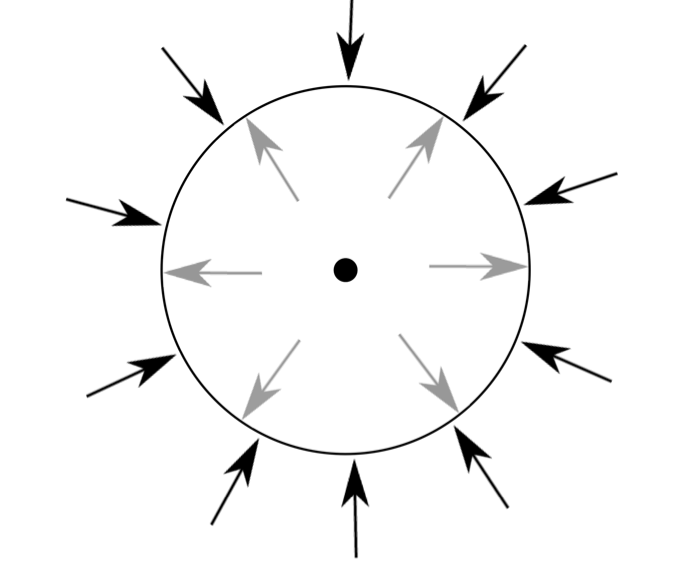
\includegraphics[width=0.4\textwidth]{./Images/Bag model.png}
\caption[Diagrama de bolsa]{\emph{Diagrama de bolsa, en el interior de la bolsa tenemos la presión generada por un plasma de quarks y gluones que considera tanto la presión dada por los quarks, por los gluones y por la interacción entre estos (dentro) y por otro lado la presión hacia el interior dada por la bolsa que coincide con los límites del hadrón.}}
\label{fig: Bolsa}
\end{wrapfigure}

De esta manera, en nuestro modelo consideramos una simplificación de todos los cálculos que se ocupan en \acrshort{qcd}, con el fin de reducir esas interacciones a la contribución de una presión de bolsa $B$.

Como en el código de \ref{code:python_example}

Por otro lado, consideramos la estadística no extensiva de Tsallis ya que proporciona el modelo necesario para representar al plasma de quarks y gluones (visto como gases de Fermi y Dirac por simplificación) con un parámetro que considera la interacción entre los quarks y los gluones. Este modelo se ha escogido por sus varias aplicaciones en otras áreas de investigación [más referencias] y que se ajusta muy bien a este modelo por tratarse de partículas que interaccionan y con ello simplifican la no linearidad propia de esto [más referencias]. Cabe mencionar, que en este marco se pueden considerar gases con potencial químico, $\mu$, no nulo lo cual es una ventaja a la hora de estudiar los diversos escenarios en los que los hadrones se encuentran.

%Here, we propose a phenomenological description based on the MIT bag model [10,11] and a non-extensive statistical approach. This could be referred to as the T-MIT bag model to abbreviate the merger of Tsallis non-extensive statistics and the MIT Bag Model [12].

Aquí proponemos una descripción fenomenológica basada en el modelo de bolsa del MIT \cite{Chodos_1974,Chodos1974a} y una aproximación estadística no extensiva. Esta podría ser referida como \acrshort{t-mitbm} para abreviar la unión de la estadística no extensiva de Tsallis y el \acrshort{mit} \acrshort{bm} \cite{Barboza_Mendoza_2019}

De esta manera, el modelo \acrshort{t-mitbm} es un modelo que introduce un potencial químico, $\mu$, distinto de cero para estudiar el modelo hadrónico un poco más extendido. Hemos comparado estos resultados con los obtenidos en [Nature], donde se ha obtenido la distribución de presión de quarks dentro del protón usando \acrfull{dvcs}, lo cual consiste en dispersar fotones virtuales de altas energías radiadas por electrones y la emisión subsecuente de un protón real. El fotón en el estado final permite la estimación de transferencia de momento al protón, que permanece intacto. El análisis recae en métodos desarrollados para extraer información a partir de \acrfull{gpd} y \acrfull{cff}. Así se obtuvo una presión repulsiva de los quarks cerca del centro del protón y una presión de atadura a distancias por encima de $0.6 \, \mathit{\unit{\femto\meter}}$ del centro. Sin embargo, hay que recordar que esto solo corresponde a los quarks, la presión debido a los gluones no se considera.

NOTA: Agregar referecnias respecto a resultados experimentales acerca de la presión dentro del protón y la estructura del hadron.

%Tsallis statistics was introduced as a generalization of the Boltzmann–Gibbs statistics approach [13–17]. The Tsallis statistic has been widely used in high-energy physics. It was introduced for the first time to describe particle production in electron–positron collisions. The differential distributions of transverse momenta for charged hadrons with respect to the jet axis at several center-of-mass energies were successfully adjusted with a Tsallis function [18,19]. Tsallis distributions have also been used in proton–proton [20–23] and heavy ion [24,25] collisions to describe the experimental data. The observed success in describing the experimental data indicates that some underlying physics may be at work at a more fundamental level.

La estadística de Tsallis fue introducida como una generalización de la aproximación de \acrshort{bg} \cite{Tsallis1988,Beck_2003,Tsallis2009,Tsallis_2014,Tsallis_2009}. La estadística de Tsallis ha sido ampliamente usada en física de altas energías. Fue introducida por primera vez para describir producción de partículas en colisiones electrón positrón. Las distribuciones diferenciales de momento transversal para hadrones cargados con respecto al eje de jet en varias energías de centro de masa fueron ajustadas existosamente con una función de Tsallis \cite{Bediaga_2000,Collaboration1984}. Las distribuciones de Tsallis también han sido usadas en colisiones protón protón\cite{PhysRevLett.105.022002,Marques_2015,Bhattacharyya_2018,Khuntia_2017} y iones pesados \cite{Saraswat_2018,Saraswat_2017}
 para describir los datos experimentales.

%Here, we incorporate the non-extensive Tsallis statistics in the MIT bag model to describe fermions and bosons as non-independent components of hadrons. In the new T-MIT bag model, one can estimate the total pressure distribution inside nucleons. We compared the resulting profile with the extracted pressure distribution of quarks published recently [26].

Aquí, incorporamos la estadística no extensiva de Tsallis en el \acrshort{t-mitbm} para describir fermiones y bosones como componentes no independientes de los hadrones. En el nuevo \acrshort{t-mitbm}, uno puede estimar la distribución de presión total dentro de los nucleones. Comparamos el perfil resultante con la distribución de presión extraida de quarks publicada recientemente \cite{Burkert_2018}.

%On the experimental side, projects are now implementing techniques to gain more insight into the hadron structure [27], as well as the residual effects of strong nucleon- nucleon and nucleon–hyperon interactions [28,29]. The Electron Ion Collider (EIC) [30] planned for construction at Brookhaven National Laboratory will be dedicated to unrav- elling details of the strong interaction. It probes the transition between the perturbative and non-perturbative phenomena of QCD and the internal structure of protons and atomic nuclei. The EIC will reveal features of the sea of quark-antiquark pairs and key aspects of the gluon distribution. Effective models will continue to provide guidelines. The model proposed here offers a new approach to look at the structure of hadrons. We are not aware of similar advances aimed at estimating the pressure inside hadrons, although the fusion of the MIT bag model and Tsallis statistics has been performed previously [31,32].

Por el lado experimental, los proyectos están ahora implementando técnicas para ganar más conocimiento en la estructura del hadrón\cite{PhysRevLett.100.162002} así como los efectos residuales de interacciones fuertes nucleon nucleon y nucleon hiperon \cite{Collaboration2015,Mihaylov_2021}. El colisionador de iones de electrones 

En el trabajo que se describe a continuación tenemos la siguiente estructura: En el capítulo \ref{ch-BagModel} se explica a detalle el modelo de bolsa que hemos ocupado en este trabajo, se explica por qué es útil el modelo de bolsa, sus limitaciones y se desarrollan las ecuaciones necesarias para hallar la presión de bolsa y una breve explicación de cómo es que se puede interpretar, en una sección posterior se busca darle otra interpretación; el capítulo \ref{ch-Tsallis} hace una explicación detallada de cómo se tratan los quarks y los gluones dentro de los hadrones y cómo es que la no extensitividad produce un parámetro de Tsallis $q$, tal que sustituye la interacción entre quarks y gluones y explica por qué es una extensión de la estadística de \acrfull{bg}: el capítulo 4 trata de un último preámbulo y es que hemos considerado que la temperatura, parámetro necesario para hallar la presión dentro de la estadística de Tsallis, es función de la distacia respecto al origen de nuestro hadrón; el capítulo 5 explica primeramente los resultados obtenidos en [Nature] y cómo se obtiene la distribución de presión de quarks usando \acrshort{dvcs}, y a partir de nuestro marco \acrshort{t-mitbm} encontramos la presión de gluones, se muestran algunos ejemplos de cómo varía a distintos valores de potencial químico, $\mu$, y se compara con la presión de quarks de nature y la presión total; el capítulo 6 habla de una posible interpretación física del parámetro de Tsallis $q$, y su relación con la presión de bolsa; finalmente en el capítulo 7 comparamos nuestros resultados obtenidos con el modelo \acrshort{t-mitbm} y esos de [Nature]

\newpage

\thispagestyle{empty}